% Cal Poly Thesis
% 
% based on UC Thesis format
%
% modified by Mark Barry 2/07.
%




\documentclass[12pt]{ucthesis}

\newif\ifpdf
\ifx\pdfoutput\undefined
    \pdffalse % we are not running PDFLaTeX
\else
\pdfoutput=1 % we are running PDFLaTeX
\pdftrue \fi

\usepackage{url}
\ifpdf

    \usepackage[pdftex]{graphicx}
    % Update title and author below...
    \usepackage[pdftex,plainpages=false,breaklinks=true,colorlinks=true,urlcolor=blue,citecolor=blue,%
                                       linkcolor=blue,bookmarks=true,bookmarksopen=true,%
                                       bookmarksopenlevel=3,pdfstartview=FitV,
                                       pdfauthor={!!Author goes here!!},
                                       pdftitle={!!Title goes here!!},
                                       pdfkeywords={thesis, masters, cal poly}
                                       ]{hyperref}
    %Options with pdfstartview are FitV, FitB and FitH
    \pdfcompresslevel=1

\else
    \usepackage{graphicx}
\fi

\usepackage{amssymb}
\usepackage{amsmath}
\usepackage[letterpaper]{geometry}
\usepackage[overload]{textcase}



\bibliographystyle{abbrv}

\setlength{\parindent}{0.25in} \setlength{\parskip}{6pt}

\geometry{verbose,nohead,tmargin=1.25in,bmargin=1in,lmargin=1.5in,rmargin=1.3in}

\setcounter{tocdepth}{2}


% Different font in captions (single-spaced, bold) ------------
\newcommand{\captionfonts}{\small\bf\ssp}

\makeatletter  % Allow the use of @ in command names
\long\def\@makecaption#1#2{%
  \vskip\abovecaptionskip
  \sbox\@tempboxa{{\captionfonts #1: #2}}%
  \ifdim \wd\@tempboxa >\hsize
    {\captionfonts #1: #2\par}
  \else
    \hbox to\hsize{\hfil\box\@tempboxa\hfil}%
  \fi
  \vskip\belowcaptionskip}
\makeatother   % Cancel the effect of \makeatletter
% ---------------------------------------




\begin{document}

% Declarations for Front Matter

% Update fields below!
\title{This is the Title of My Thesis}
\author{John Smith}
\degreemonth{February} \degreeyear{2009} \degree{Master of Science}
\defensemonth{February} \defenseyear{2009}
\numberofmembers{3} \chair{Zo\"{e} Wood, Ph.D.} \othermemberA{Chris Clark, Ph.D.} \othermemberB{Chris Buckalew, Ph.D.} \field{Computer Science} \campus{San Luis Obispo}
\copyrightyears{seven}



\maketitle

\begin{frontmatter}

% Custom made for Cal Poly (by Mark Barry, modified by Andrew Tsui).
\copyrightpage

% Custom made for Cal Poly (by Andrew Tsui).
\committeemembershippage

\begin{abstract}

This is where the abstract goes.  Hopefully this document will serve as an example for preparing a Cal Poly Master's thesis.  It was thrown together pretty quickly.  A lot more neat LaTeX features, help, and examples can be found on the web.  Here is one: http://en.wikibooks.org/wiki/LaTeX

For developing LaTeX documents in the Windows environment, I use TeXnicCenter (http://www.toolscenter.org/).  A simple WYSIWYG LaTeX editor (though I had problems getting it to work with this thesis format) is \textbf{LyX} (http://www.lyx.org/).

I use \textbf{InkScape} (http://www.inkscape.org/) to create any drawings/figures needed.  It is a free vector graphics editor that is very powerful and popular.  There is an example figure produced with InkScape in Figure~\ref{fig:inkscape-example}.  InkScape can export images in many different formats.  Export your images as PDF or EPS and put into your LaTeX document.  If you're creating a PDF document with \textbf{pdflatex}, then export as a PDF image.  If you're creating PostScript then export as EPS.  Rasterized images such as JPEG can also be easily included in LaTeX.

LaTeX can also produce nice equations.  Did you know that $\sum_{n=0}^{\infty} \frac{(-1)^n}{2n+1} = \frac{1}{1} - \frac{1}{3} + \frac{1}{5} - \frac{1}{7} + \frac{1}{9} - \cdots = \frac{\pi}{4}$ ?  A non-inline equation can be found in Figure~\ref{eqn:example}.  I treated my equations as figures but they can be treated specially as Equations.

An example of a table can be found in Table~\ref{table:performance}.

The bibliography section is very easy to create.  When gathering references, I used the ACM digital library (http://portal.acm.org/portal.cfm) to grab the Bibtex entries.  Papers in the digital library have Bibtex entries ready to be copied and pasted into your bibliography.  Create a separate file called something like ``bibliography.bib'' and paste in your Bibtex entries.  LaTeX (and Bibtex) generate your bibliography section for you -- very easy! I can cite references very easily.  Here is a paper called \emph{Dual contouring of hermite data}~\cite{DualContouring}.  Here is a paper called \emph{Surface simplification using quadric error metrics}~\cite{QuadricErrorMetrics}.  I've also cited software located at some websites \cite{NormalMapper}~\cite{nVidiaMelody}.


\end{abstract}

%\begin{acknowledgements}

%   Thank you...

%\end{acknowledgements}


\tableofcontents


\listoftables

\listoffigures

\end{frontmatter}

\pagestyle{plain}




\renewcommand{\baselinestretch}{1.66}


% ------------- Main chapters here --------------------


\chapter{Introduction}
\label{intro}

Human brains are built to come to single conclusions about things that have more than one interpretation.  The way that you come to this end conclusion is dependent upon your experiences, cutural immersion, and language familiarity \cite{smith_music_2003}. When attempting to write English phrases that will be read aloud and heard by people with other linguistic biases than you, it's important to make your prose as deterministically understandable as possible. The first step towards this is understanding and identifying how many ways a particular textual phrase be misheard, and why.


\section{You and me...and Leslie?}
\label{sect:youAndMeAndLeslie}

In the song \textit{``Groovin' (on a Sunday Afternoon)''}, by the Young Rascals, there's a part in the bridge that many people hear as \textit{``Life would be ecstasy, you an' me an' Leslie''}. In fact, the line is \textit{``Life would be ecstasy, you and me endlessly''}. The confusion lies with the last three syllables of the phrase. The pronunciation of each version, if spoken normally, is as follows:



%\begin{table}
\begin{center}
    \begin{tabular}{|l|c|c|}
        \hline
        \textbf{Orthographic:} & and       Les-   lie & end-       less-       ly \\ 
        \hline
        \textbf{SAMPA:}      & @nd   ``lEs     li   & ``End      l@s       li   \\
        \hline
    \end{tabular}
\label{table:groovinAlphaSAMPA}
\end{center}
%\end{table}


In the song, the singer is doing what many singers are taught to do, to make it easier to sustain the singing of words that end with difficult-to-sing consonants: the unsingable consonant is displaced onto the front of the next word. In this case, the consonant ``d'' is not singable, so he displaces it onto the next syllable, when he can: ``and ME'' becomes ``an dME'', and ``end LESS'' becomes ``en dLESS''. 

Basically, singers are *born* to ignore syllable boundries. So, our singer can effectively think of the sung phrase as:

\begin{center}
YOU an dME en dLESS lee
\end{center}

This does not cause confusion for listeners, because they are used to hearing it. This does mean, however, that lyric placement does not provide an accurate barometer to a listener of where a word actually ends.

In addition, the singer is singing fudging his vowels, like singers are taught to do, so ``and'' and ``end'' sound almost indistinguishable. So, really, what listeners are hearing is this:

\begin{center}
YOU en dME en dLESS lee
\end{center}

 Now, the listener's brain has to take this syllabic gobbledy-gook, and parse it into something useful. They've currently got this mess to deal with (represented in SAMPA syllables):

\begin{center}
{\large \textit{\textbf{ju }}}{\large \textit{En }}{\large \textit{\textbf{dmi 
}}}{\large \textit{En }}{\large \textit{\textbf{dl@s }}}{\large \textit{li}}
\end{center}

 They parse the first part just fine, because the emphases match:

\begin{center}
{\large \textbf{you }}{\large and }{\large \textbf{me }}{\large \textit{En }}{\large \textit{\textbf{dl@s 
}}}{\large \textit{li}}
\end{center}

But no one says endLESSly. People say ENDlessly. So, the listeners don't recognize it. They have to work with what they have. They already turned one ``En d'' into an ``and'', so they do it again:

\begin{center}
{\large \textbf{you }}{\large and }{\large \textbf{me }}{\large and }{\large \textit{\textbf{l@s 
}}}{\large \textit{li}}
\end{center}

Now, they're just left with LESS lee. And that fits Leslie, a proper noun that fits in context and in emphasis placement. So, the final heard lyric is:

\begin{center}
{\large \textbf{you }}{\large and }{\large \textbf{me }}{\large and }{\large \textbf{Les- 
}}{\large lie}
\end{center}

The misunderstanding can be traced back to improper emphasis placement. The songwriter probably didn't even think of that, and now he's stuck: a one-hit-wonder with a misunderstood song. We bet that in interview after interview, someone asks him who Leslie is. It's probably very frustrating --- especially since he could have just moved the word an eight note later, and it would have been understood perfectly.

That's the sort of situation this program is going to help avoid.



\section{ Why it breaks down }
\label{sect:whyItBreaksDown}

There are two points at which the author's intendeded phrasing can be muddled : First, when the author's orthographic text becomes an orator's spoken (phonetic) interpretation, and second, when the orator's phonetic interpretation is translated phonetically by an audience into a perceived orthographic phrase. Both of these interpretations must be made succesfully in order for the author's intended meaning to be conveyed.


The phrase ``iced ink" undisputedly succeeds in the first translation, but fails on the second.  Iced ink can only be pronouced one way, but it can be heard multiple ways--the most notable of which is ``I stink", not ``iced ink".

The phrase ``a nice cold hour" can fail on both parts.  First, the orator could have accidentally-capitalized the word Nice in their head, and made it sound like Nice, the city in France.  An audience would likely hear this as ``niece", and would be confused, at best.  Even if the orator pronouces the phrase as the author intended, the audience could hear multiple orthographic phrases in the same phonetic sequence: ``a nice cold hour", ``an ice cold hour", or even ``a nigh scold our".

A third, more rare and nefarious type of audience misunderstanding can be caused by parse-tree misdirection, where an audience member is absolutely sure they're hearing one phrase, only to get lost halfway through the lyric because they though they were interpreting a phonetic sequence in a way that resulted in an orthographic dead end. This happens due to the relative frequency of the possible lyrics heard.

 For example, when asked to sing along with the Adele song, Rolling in the Deep, people who were starting to sing enthusiastically dropped out around the line ``reaching a fever pitch"\cite{frontPorchBandAdeleCover}.  Let us consider the phrase ``fever pitch".  This phrase has no exact oronyms, but it does have a potential dead end-- a listener could hear the first syllable of the phrase as the word ``fee", which has a frequency of 7265.  That's more than double the frequency of the word ``fever", which is 3095.  

Looking at the oronym parse tree for the phrase ``fever pitch" in figure ~\ref{fig:feverPitchOronymTree}, we can see that the branch for ``fever" ends in a much smaller radius than the branch on the left for the word ``fee".  As you can see by the relative size of the end spheres of the branches, the word ``fee" even outweighs the last word in the other branch as well (which is ``pitch" with a frequency of 5104). Since the human brain is pre-disposed to parse more-familiar words, having that heavily-weighted dead-end branch is likely the cause of the casual listener not being able to memorize the lyrics.
\begin{wrapfigure}{r}{0.5\textwidth}[h]
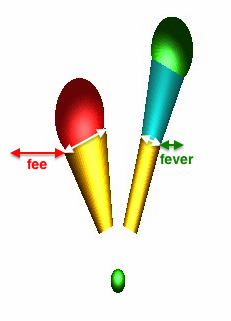
\includegraphics[width=.5\textwidth]{feverPitchTreeAnnotated.jpg}
\captionfonts
\caption[Annotated Oronym Parse tree  generated for the phrase ``fever pitch"]{ Annotated Oronym Parse tree generated for the phrase ``fever pitch" }
\label{fig:feverPitchOronymTree}
\end{wrapfigure}







\begin{figure}
\begin{center}
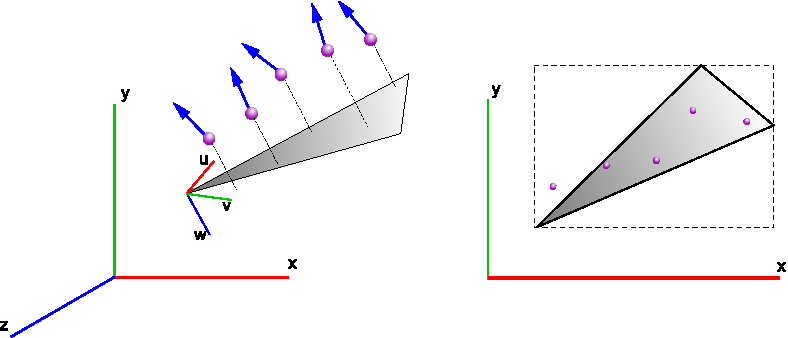
\includegraphics[height=40mm]{example_figure.pdf}
\captionfonts
\caption[This is a figure]{This is an example figure.  This graphic was drawn in InkScape (http://www.inkscape.org/), a free vector drawing application.  Figures can be exported from InkScape as PDF images or as EPS (depending upon if you want LaTeX to generate a PDF or a PostScript document.)}
\label{fig:inkscape-example}
\end{center}
\end{figure}

\chapter{Background}
\label{background}

\textcolor{Red}{I think I decimated this section when I wrote the Preliminary Vocab section.  Is there something else that should go here?}


\include{previous-work}


\begin{figure}
\begin{center}
\[
\left[\begin{array}{ccc}
u_{x} & u_{y} & u_{z}\\
v_{x} & v_{y} & v_{z}\\
w_{x} & w_{y} & w_{z}\end{array}\right]\left[\begin{array}{c}
p_{x}\\
p_{y}\\
p_{z}\end{array}\right]=\left[\begin{array}{c}
p_{x}^{\prime}\\
p_{y}^{\prime}\\
p_{z}^{\prime}\end{array}\right]\]
\captionfonts
\caption[A matrix equation]{This is a sample matrix equation.}
\label{eqn:example}
\end{center}
\end{figure}


LaTeX was originally written in 1984 by Leslie Lamport at SRI International and has become the dominant method for using TeX�few people write in plain TeX anymore.

LaTeX is based on the idea that authors should be able to focus on the meaning of what they are writing, without being distracted by the visual presentation of the information. In preparing a LaTeX document, the author specifies the logical structure using familiar concepts such as chapter, section, table, figure, etc., and lets the LaTeX system worry about the presentation of these structures. It therefore encourages the separation of layout from content, while still allowing manual typesetting adjustments where needed. This is similar to the mechanism by which many word processors allow styles to be defined globally for an entire document, or the CSS mechanism used by HTML.


\begin{enumerate}
\item Here is a list item.
\begin{enumerate}
\item Here is a sub list item.
\begin{enumerate}
\item Here is a sub sub list item.

\end{enumerate}
\end{enumerate}
\end{enumerate}


\chapter{Results}
\label{results}

\section{Phase One Results}
\label{results:userStudyPhaseOne}

In this phase, we recorded \uniqueUsersPhaseOneUserStudy users reciting any of the \numOronymsPhaseOneUserStudy  oronyms of the phrase ``an ice cold hour'', or any of the \numForthRightOohOronymPhrases oronyms for the phrase ``fourth rye to''.  Out of \numResponsesPhaseOneUserStudy recordings, only the recordings of the oronyms of ``fourth rye to" were found to diverge from our excepted phonetic patterns, likely due to poor microphone quality not being able to pick up the aspriated \emph{`f'} sound at the beginning of the phrase\cite{elko_electronic_2007}. All other oronyms were found to be within reasonable tolerance levels, with \recordingsPhaseTwoUserStudy recordings from one particular speaker found to be a close enough match to the general American accent to use his recordings in phase two.


\section{Phase Two Results}
\label{results:userStudyPhaseTwo}


We gathered \numTotalTranscriptionsPhaseTwo transcriptions for our \recordingsPhaseTwoUserStudy recorded phrases, with each recording garnering \numTranscriptionsPerRecordingPhaseTwoUserStudy transcriptions each.  Worldwide, the top four most-frequently transcribed phrases made up for 70\% of total transcriptions.  The top transcribed phrase worldwide was ``an ice cold hour'', with \phaseTwoUserStudyTimesTranscribedAnIceColdHour transcriptions, followed by  ``a nice cold hour'', with \phaseTwoUserStudyTimesTranscribedANiceColdHour transcriptions.  Following that, ``a nice gold hour'' had \phaseTwoUserStudyTimesTranscribedANiceGoldHour transcriptions, and ``in ice cold hour'' had \phaseTwoUserStudyTimesTranscribedInIceColdHour transcriptions. The breakdown of these top four can be seen in figure ~\ref{fig:mostCommonTranscriptionsPieChartGlobal} and table ~\ref{table:fullFreqVsActual}. 

All of the worldwide top transcribed phrases were predicted by our oronym-generator, except for ``a nice gold hour''.  This is a known limitation of our project, though, because we chose to focus on exact phonetic matches.  The cold/gold mishearing is a product of phoneme voiced/voiceless pair swapping, which we cover in-depth in section ~\ref{section:phonemeSwapping}. It is outside the current scope of our project. 


\begin{figure}
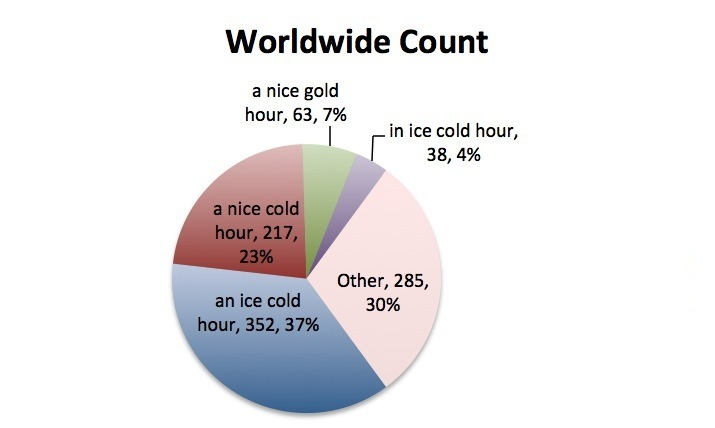
\includegraphics[width=150mm]{PieChart_WorldwideCount_noBar.jpg}
\captionfonts
\caption[Most Common Transcriptions Globally]{ Our top two transcriptions were ``a nice cold hour'' and ``an ice cold hour'' }
\label{fig:mostCommonTranscriptionsPieChartGlobal}
\end{figure}


\begin{table}
\begin{center}
\begin{tabular}{ | l | l | l | c | }
\hline 
predicted freq & phrase transcribed & total answers \\
\hline 
931028 &  an ice cold hour &  \phaseTwoUserStudyTimesTranscribedAnIceColdHour \\
\hline
7851662&   a nice cold hour &  \phaseTwoUserStudyTimesTranscribedANiceColdHour  \\
\hline
0  & a nice gold hour &  \phaseTwoUserStudyTimesTranscribedANiceGoldHour \\
\hline
5503158&   in ice cold hour &  \phaseTwoUserStudyTimesTranscribedInIceColdHour \\
\hline
0 &  an ice gold hour &  \phaseTwoUserStudyTimesTranscribedAnIceGoldHour \\
\hline
859307 &  an eye scold hour &  \phaseTwoUserStudyTimesTranscribedAnEyeScoldHour \\
\hline 
\end{tabular}
\captionfonts
\caption[Phrase word frequency sum vs times transcribed]{ In this table, we list all oronyms that were transcribed more than five times. Out of this list, all but the two containing the word ``gold" were predicted by our oronym algorithm.  However, we expected that any voiced/voiceless phoneme substitutions, like ``cold''/``gold'' would be missed by our algorithm. }
\label{table:fullFreqVsActual}
\end{center}
\end{table}


%\begin{figure}
%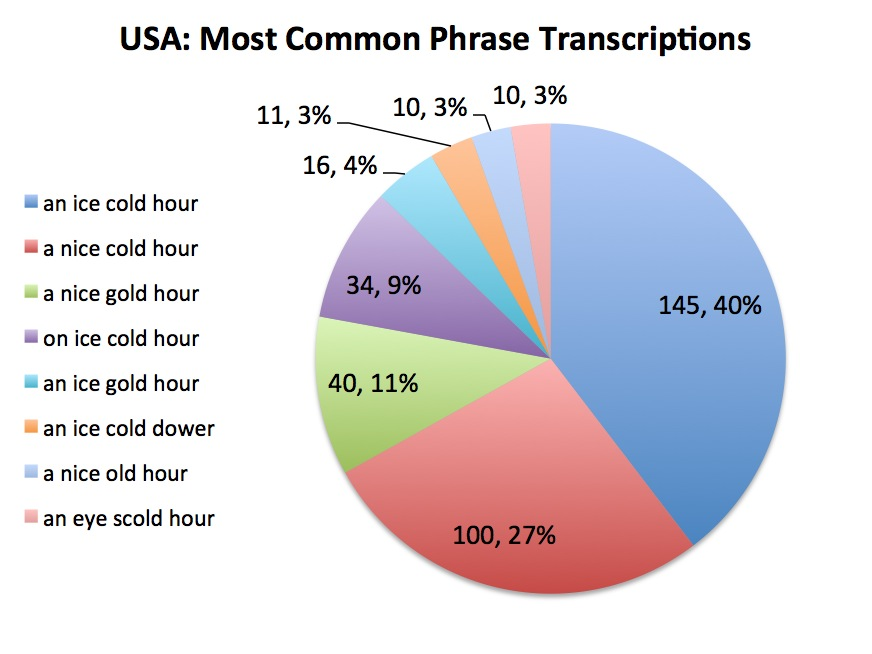
\includegraphics[width=150mm]{mostCommonTranscriptionsPieChartUSA.jpg}
%\captionfonts
%\caption[Most Common Transcriptions from American respondents]{ Though the breakdown is a bit different than the global transcription breakdown, you can still see the clear trend of ``a nice cold hour" and ``an ice cold hour" being the most common.  There is a slightly larger gap between these two phrase, we hypothesize, because the American transcribers are familiar with what words normally are in proximity to others. }
%\label{fig:mostCommonTranscriptionsPieChartUSA}
%\end{figure}



\subsection{Transcribed oronyms' observed frequency vs expected frequency}
\label{results:transcriptionExpectedVsObservedFreq}

Though the most commonly transcribed phrases were predicted by our method of oronym generation, figure ~\ref{fig:results:aNiceColdHourObserved} shows an unexpected distribution of the number of times each phrase was transcribed versus the frequency metric that we calculated. We hypothesized that a simple summation of the UNISYN-provided word frequencies for each word in a phrase would produce a meaningful indicator of whether a phrase's likelyhood to be heard.  

\begin{figure}
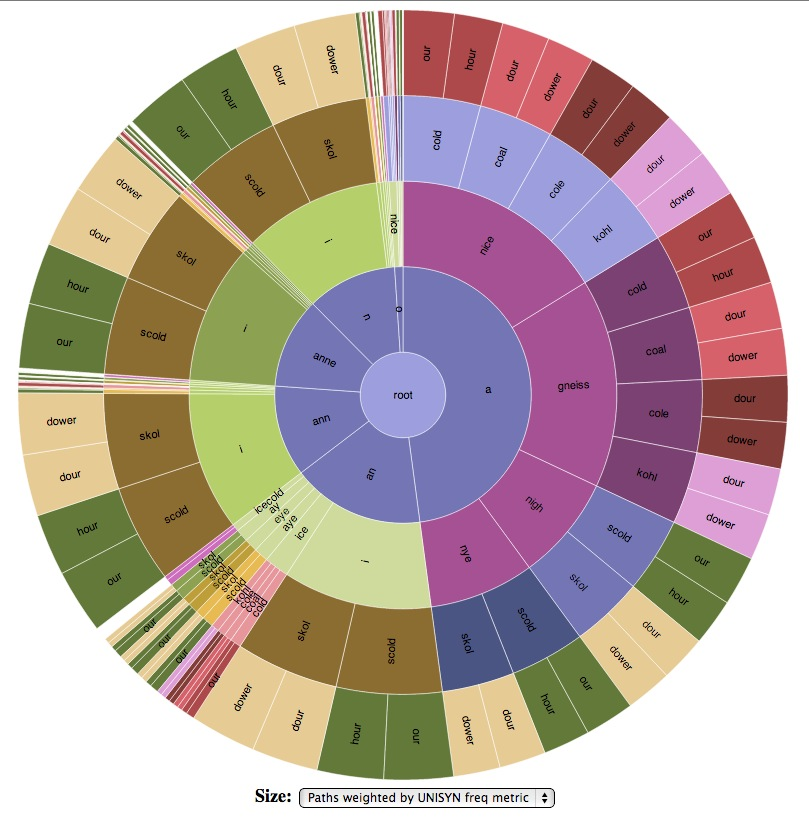
\includegraphics[width=150mm]{aNiceColdHour_UNISYN_FreqMetric_withUnpredictedSliver.jpg}
\captionfonts
\caption[Sunburst Chart for A Nice Cold Hour using UNISYN metrics for comparison to observed frequency sunburst]{Sunburst Chart for A Nice Cold Hour using UNISYN metrics for comparison to observed frequency sunburst}
\label{fig:results:aNiceColdHourUNISYNwithUnpredicted}
\end{figure}

\begin{figure}
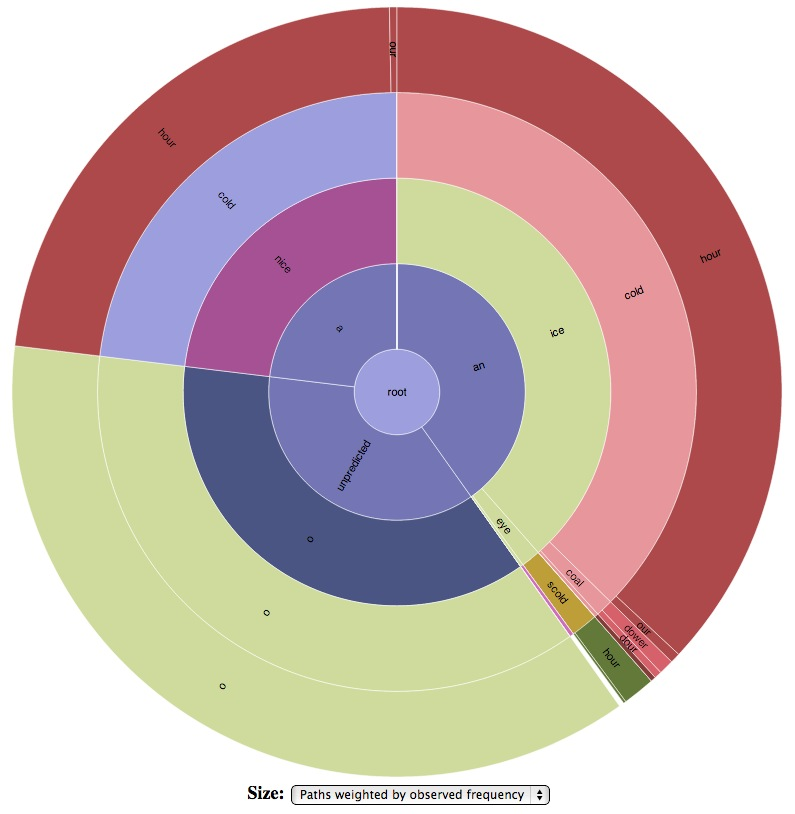
\includegraphics[width=150mm]{aNiceColdHour_Observed.jpg}
\captionfonts
\caption[Sunburst Chart for A Nice Cold Hour using observed frequencies]{Sunburst Chart for A Nice Cold Hour using observed frequencies}
\label{fig:results:aNiceColdHourObserved}
\end{figure}


Unfortunately, that proved not to be the case.  In figure ~\ref{fig:results:aNiceColdHourUNISYNwithUnpredicted}, we see the sunburst diagram for the expected distribution of transcribed phrases based upon the UNISYN frequency metric that we calculated.  In figure ~\ref{fig:results:aNiceColdHourObserved}, we see the sunburst diagram for the transcriptions we observed, with a special slice representing all the transcriptions we did not predict. The unpredicted slice is nearly as large as the slice for ``an ice cold hour'', which was observed the most often out of all expected transcriptions. 


\subsection{Statistical measurement of expected versus observed transcription frequency}
\label{results:statisticsINYOURFACE}


A statistical analysis of the observed dataset versus the expected dataset, using a one-proportion z test, further proves that the calculated UNISYN frequency values were not a good predictor of observed transcription.   Using the top two observed transcriptions as our sample population, we take a look at the phrases \phraseOne and \phraseTwo.  The phrase \phraseOne has a calculated UNISYN freq metric of \unisynFreqForPhraseOne, and had \USATranscriptionsOfPhraseOne actual transcriptions observed among people living in the United States. The phrase \phraseTwo has a calculated UNISYN freq metric of \unisynFreqForPhraseTwo, and had \USATranscriptionsOfPhraseTwo actual transcriptions observed among people living in the United States. Therefore, the expected population is \unisynCombinedFreq, and the observed population is \USACombinedTranscriptions.  

Given those population, the expected population proportion for \phraseOne would be \unisynFreqForPhraseOne  $\div$ \unisynCombinedFreq, or \expectedProportionOfPhraseOneOccurances.  

In our user study, we found that \USATranscriptionsOfPhraseOne people transcribed \phraseOne, and \USATranscriptionsOfPhraseTwo people transcribed \phraseTwo, for a ratio of 0.65 to 1, where \phraseOne accounts for 39.56\% ( p = \observedProportionOfPhraseOneOccurances ) of the combined count. 

Given the observed population proportion of \observedProportionOfPhraseOneOccurances and the expected population proportion \expectedProportionOfPhraseOneOccurances, we did a one-proportion z test with an $\alpha$ of \alphaSigFigs.  The z value returned was \UNISYNzVal, meaning that the observed population proportion was \UNISYNzVal standard deviations away from the expected population proportion.  When we used this z value to compute a p value, we got a value so low that we were unable find a calculator with enough decimal places to show it without rounding it to zero.

In short, the per-occurance frequency metric predictions derived from UNISYN don't even remotely match the observed data.


The below is here mostly for my edification: (I'll delete it when my edits are all done.)

Givens for Phrase (1) (\phraseOne) :

Calculated metric: \unisynFreqForPhraseOne

Actual count: x = \USATranscriptionsOfPhraseOne


Givens for Phrase (2) (\phraseTwo) :

Calculated metric: \unisynFreqForPhraseTwo

Actual count: x = \USATranscriptionsOfPhraseTwo

$\alpha$ = significance Level = \alphaSigFigs

Calculated sum: \unisynFreqForPhraseOne + \unisynFreqForPhraseTwo =  \unisynCombinedFreq

Actual sum: \USATranscriptionsOfPhraseOne + \USATranscriptionsOfPhraseTwo = \USACombinedTranscriptions

p = population proportion of \phraseOne occurrences

p = \unisynFreqForPhraseOne   $\div$  \unisynCombinedFreq  = \pvalue 

$H_{o}$ :  p = \pvalue 
$H_{a}$ :  p $\neq$ \pvalue 

Actual: 
\USATranscriptionsOfPhraseOne  $\div$ \USACombinedTranscriptions  = 

1-proportion z-test

z = \UNISYNzVal std deviations away from expected.

If pvalue < $\alpha$, reject $H_{o}$

pvalue $\approx$ 0 < \alphaSigFigs

So, reject $H_{o}$


\subsection{Observations on Transcription Count per Recording for each transcribed phrase}
\label{results:transcriptionCountPerRecording}

The Transcription Count by Recording graphs show how many occurances of a certain transcription were produced from each recording. Each graph represents one transcription, and has bars for each recording, where each bar shows how many times the transcription was observed for that particular recording. The graph also compares the observed incidences of those transcriptions with the expected UNISYN frequency metric. The X axis lists the transcribed phrase.  The right Y axis corresponds to the smaller, multi-colored bars. Each bar represents the number of times that a transcribed phrase was observed for that particular recording. 
The left X axis corresponds to the large blue bar behind the smaller bars. The blue bar represents the calculated UNISYN frequency metric for the transcription.


When you compare the bars from the two y axes, some interesting patterns appear. 

\subsubsection{An ice cold hour}
\label{results:transcriptionCountPerRecording:an_ice_cold_hour}

When looking at figure ~\ref{fig:results:transcriptionCountPerRecordingAnIceColdHour}, we notice that all but 12 out of the 362 transcriptions of ``an ice cold hour'' come from recordings of phrases that similarly begin with ``an''. This suggests the existence of some un-measured value related to pronunciation that makes the theoretically identical phonetic sequences of ``an ice cold hour'' and ``a nice cold hour'' be heard as functionally different. Also, note that in figure ~\ref{fig:results:transcriptionCountPerRecordingAnIceColdHour}, the blue bar representing the UNISYN frequency prediction for the transcribed phrase underpredicts the number of transcriptions from recordings that begin with ``an'', while doing a fairly good job of predicting transcription incidence for recordings that begin with ``a''.


\begin{figure}
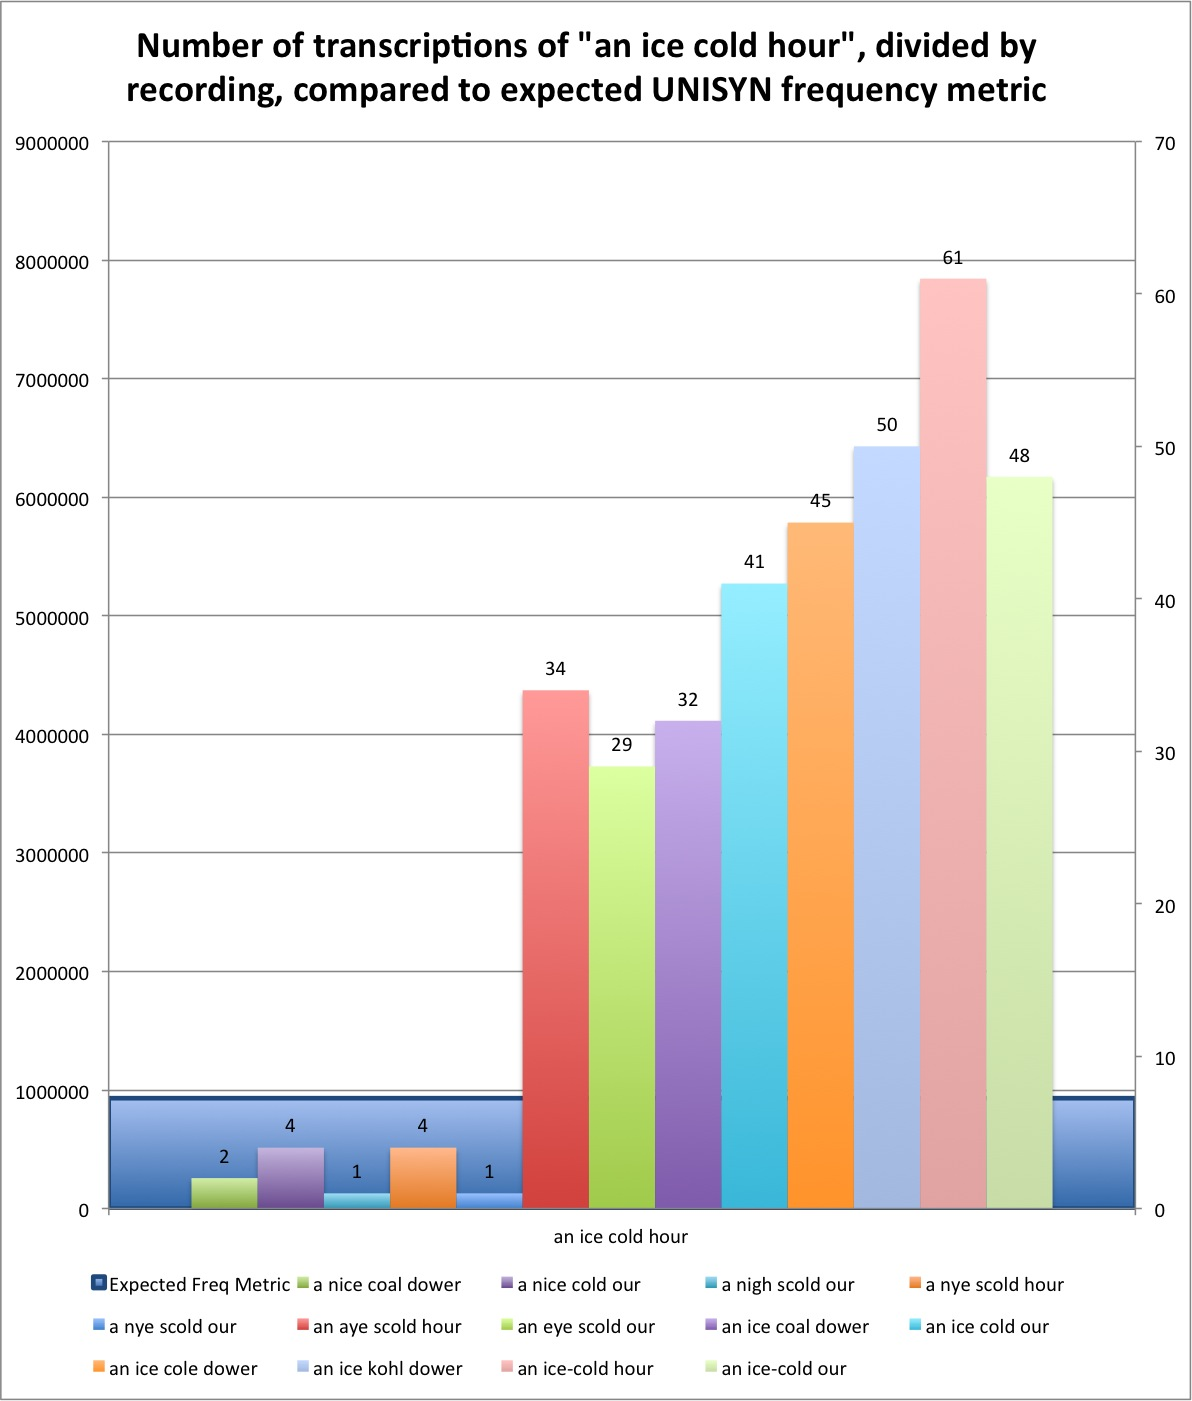
\includegraphics[width=\textwidth]{TranscriptionCountPerRecording_an_IceColdHour.jpg}
\captionfonts
\caption[Transcription Count Per Recording for the transcribed phrase ``an ice cold hour'']{ This graph represents all transcriptions of the phrase ``an ice cold hour'', divided into columns based on what recording were transcribed as ``an ice cold hour''. The large blue bar in the background shows the predicted frequency metric for the phrase in question.}
\label{fig:results:transcriptionCountPerRecordingAnIceColdHour}
\end{figure}

\subsubsection{A nice cold hour}
\label{results:transcriptionCountPerRecording:a_nice_cold_hour}

In figure ~\ref{fig:results:transcriptionCountPerRecordingANiceColdHour}, we see that, while most of the transcriptions of ``a nice cold hour'' came from recordings of phrases that begin with 'a', a not-inconsiderable number came from the recordings for the phrases ``an ice cold our'' and ``an ice-cold our''. When taken in regards to the conclusions we drew from figure ~\ref{fig:results:transcriptionCountPerRecordingAnIceColdHour} in section ~\ref{results:transcriptionCountPerRecording:an_ice_cold_hour}, we can conclude that, while listeners appear not to be able to hear an `a' as an `an', listeners can, under certain circumstances, hear an `an' as an `a'.  The blue prediction bar shows that the expected incidence over all recordings was much higher than the observed incidence, and only came close to being correct for the recorded phrases ``a nice cold hour'' and ``a nice coal dower''.

\begin{figure}
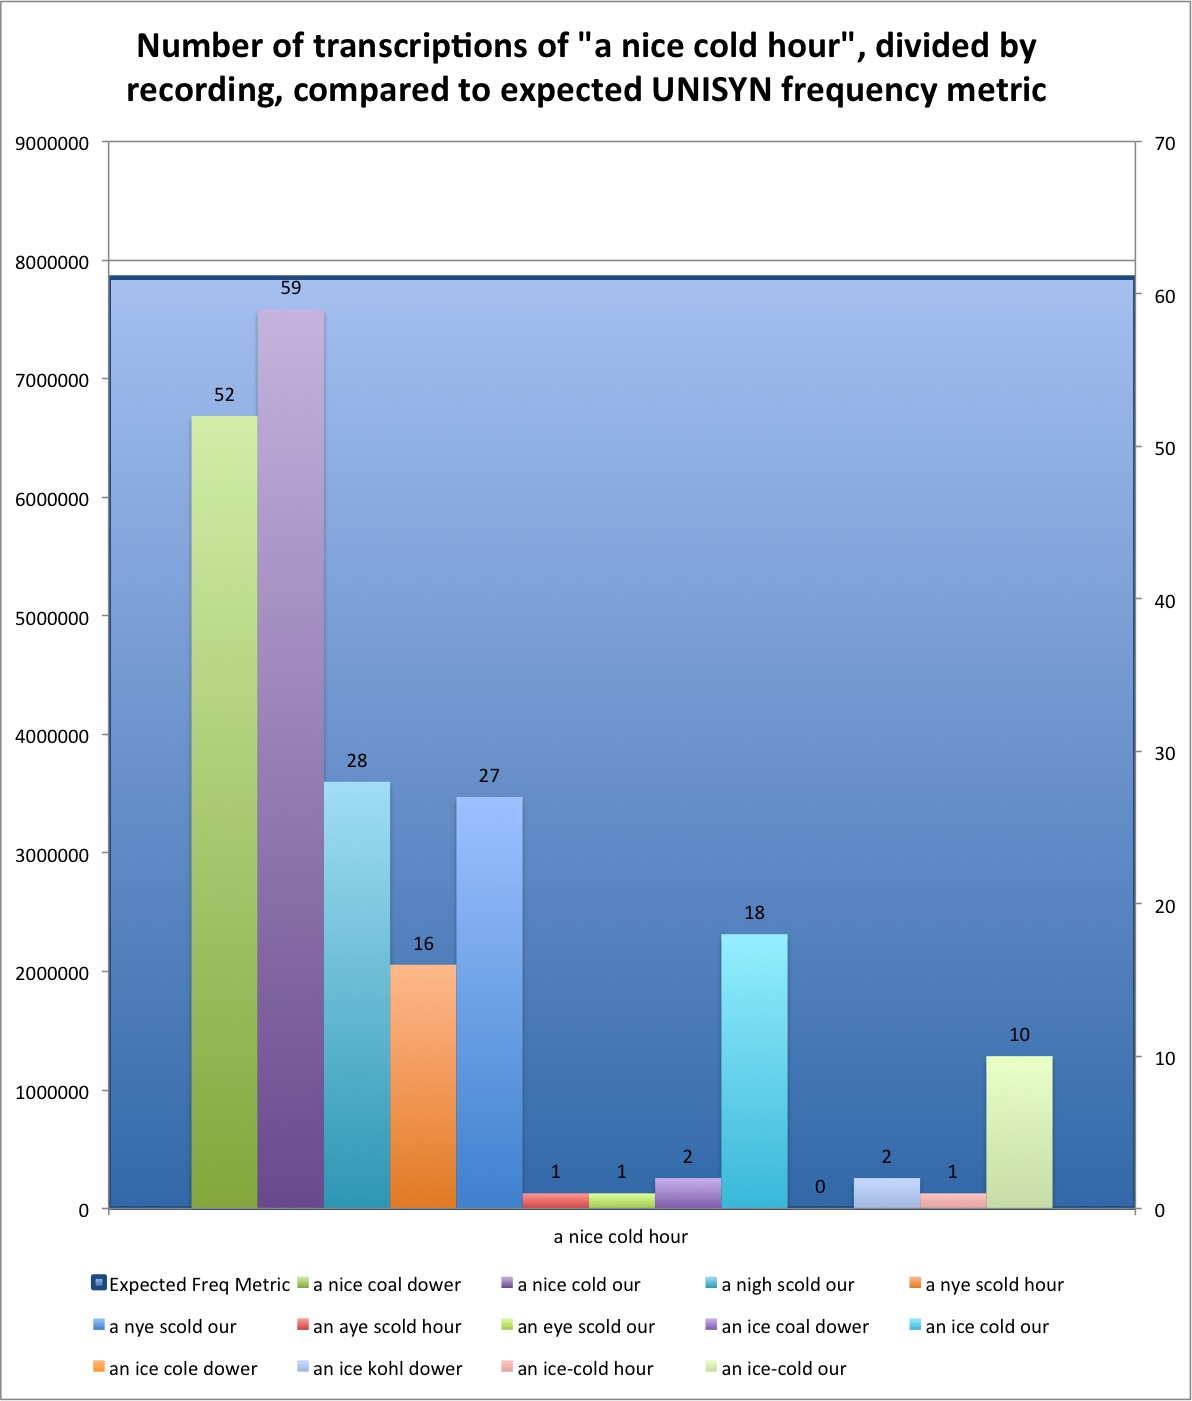
\includegraphics[width=\textwidth]{TranscriptionCountPerRecording_a_NiceColdHour.jpg}
\captionfonts
\caption[Transcription Count Per Recording for the transcribed phrase ``a nice cold hour'']{ This graph represents all transcriptions of the phrase ``a nice cold hour'', divided into columns based on what recording were transcribed as ``a nice cold hour''. The large blue bar in the background shows the predicted frequency metric for the phrase in question.}
\label{fig:results:transcriptionCountPerRecordingANiceColdHour}
\end{figure}



\subsubsection{In ice cold hour}
\label{results:transcriptionCountPerRecording:in_ice_cold_hour}

This chart in figure ~\ref{fig:results:transcriptionCountPerRecordingInIceColdHour} is for the third most common transcription, ``in ice cold hour''.  Transcriptions of this phrase are fairly evenly distributed among the recordings, though there is a spike of transcriptions on  ``an ice-cold hour''.  Additionally, similar to earlier observations, the transcriptions occur a lot less frequently than the UNISYN frequency metric bar suggests they should.

\begin{figure}
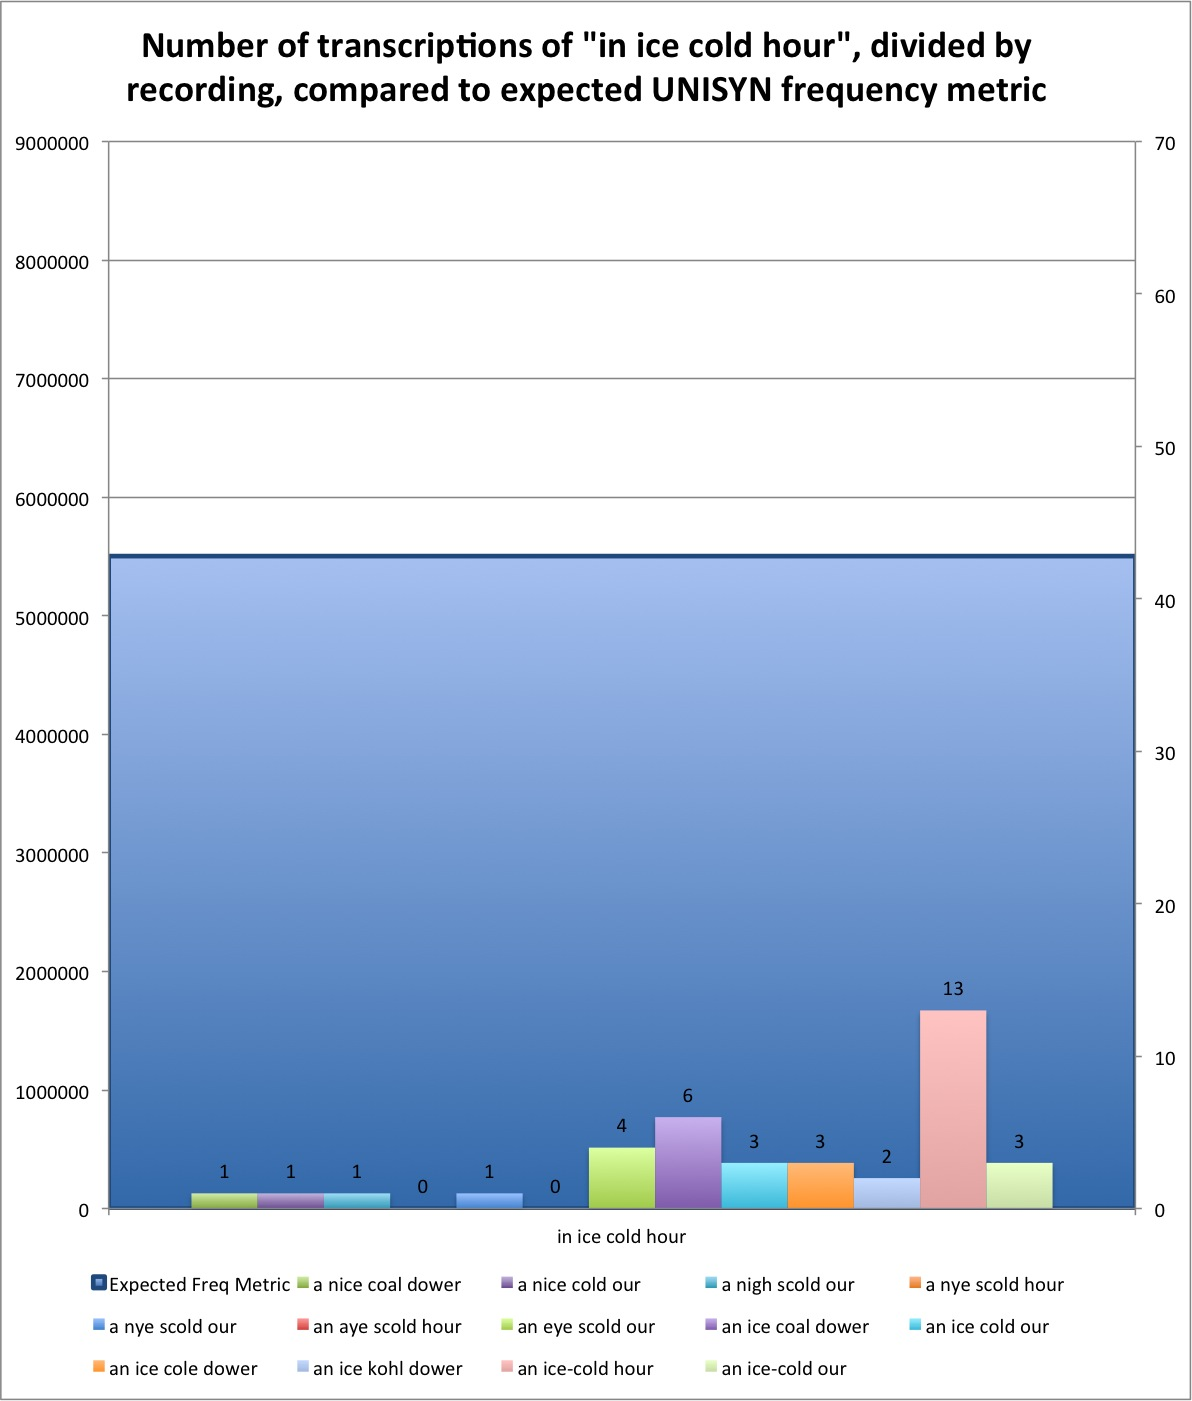
\includegraphics[width=\textwidth]{TranscriptionCountPerRecording_inIceColdHour.jpg}
\captionfonts
\caption[Transcription Count Per Recording for the transcribed phrase ``in ice cold hour'']{ This graph represents all transcriptions of the phrase ``in ice cold hour'', divided into columns based on what recording were transcribed as ``in ice cold hour''. The large blue bar in the background shows the predicted frequency metric for the phrase in question.}
\label{fig:results:transcriptionCountPerRecordingInIceColdHour}
\end{figure}



\subsubsection{A nice gold hour}
\label{results:transcriptionCountPerRecording:a_nice_gold_hour}

The chart in figure ~\ref{fig:results:transcriptionCountPerRecordingANiceGoldHour} for the transcriptions of ``a nice gold hour'' shows that the source recordings of those transcriptions are very specific: only the recordings of ``a nye scold our'', ``a nye scold hour'', and ``a nigh scold our'' produce the 'g'/'c' substitution. In fact, all of our transcriptions that involved the word ``gold'' arose from these recordings. This suggests a relationship between the phonemes \texttt{s k} and \texttt{g}, and warrants further investigation, as suggested later in section ~\ref{section:phonemeSwapping}. As shown by the lack of a background blue bar in this diagram, this transcription was not predicted by our oronym generation algorithm, due to the aforementioned phoneme swapping.

\begin{figure}
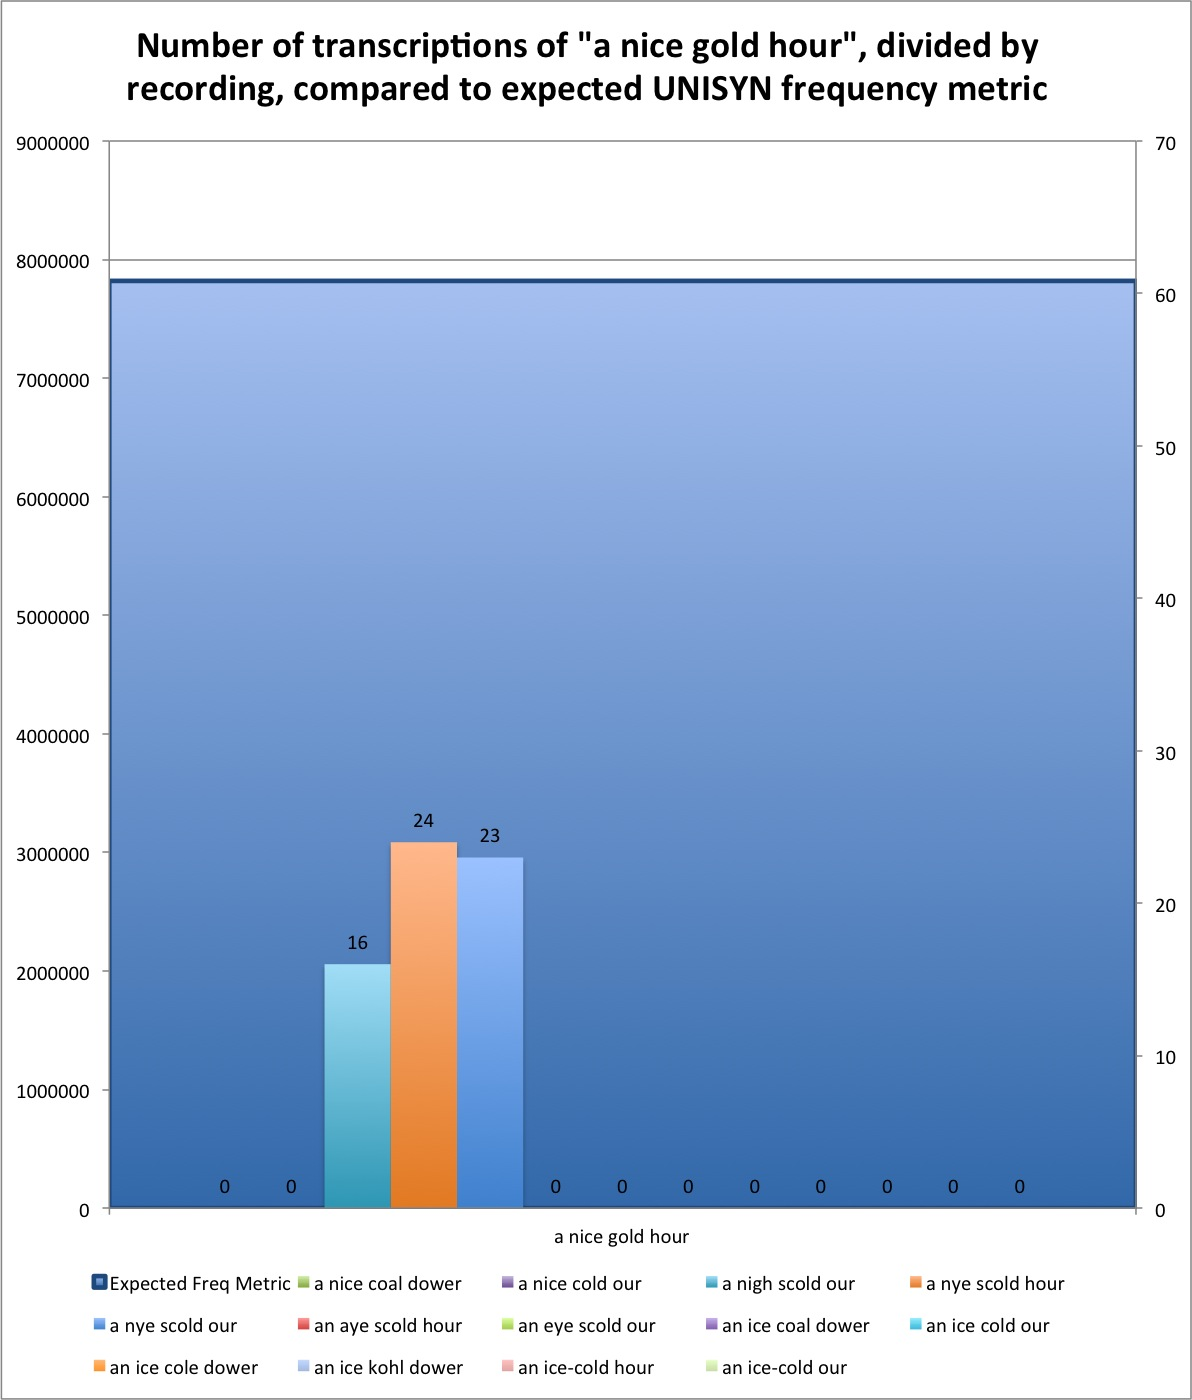
\includegraphics[width=\textwidth]{TranscriptionCountPerRecording_aNiceGoldHour.jpg}
\captionfonts
\caption[Transcription Count Per Recording for the transcribed phrase ``a nice gold hour'']{ This graph represents all transcriptions of the phrase ``a nice gold hour'', divided into columns based on what recording were transcribed as ``a nice gold hour''. The large blue bar in the background shows the predicted frequency metric for the phrase in question.}
\label{fig:results:transcriptionCountPerRecordingANiceGoldHour}
\end{figure}


\subsubsection{An ice cold dower}
\label{results:transcriptionCountPerRecording:an_ice_cold_dower}

Figure ~\ref{fig:results:transcriptionCountPerRecordingANiceColdDower} shows the transcriptions for the phrase ``an ice cold dower''. This phrase features repeated-phoneme auto-deletion or auto-insertion. Repeated-phoneme auto-deletion or -insertion occurs when two identical and adjacent phonemes are blurred into one sound.  This can result in the listener putting two phonemes where only one exists (as in this case), or putting one phoneme where two exist. This phenomenon, while known to us, is outside the scope of the current project, and suggested for future work.  Due to this limit in scope, this transcription was not predicted by our oronym generation algorithm, as shown by the lack of a background blue frequency prediction bar in figure ~\ref{fig:results:transcriptionCountPerRecordingANiceColdDower}.

\begin{figure}
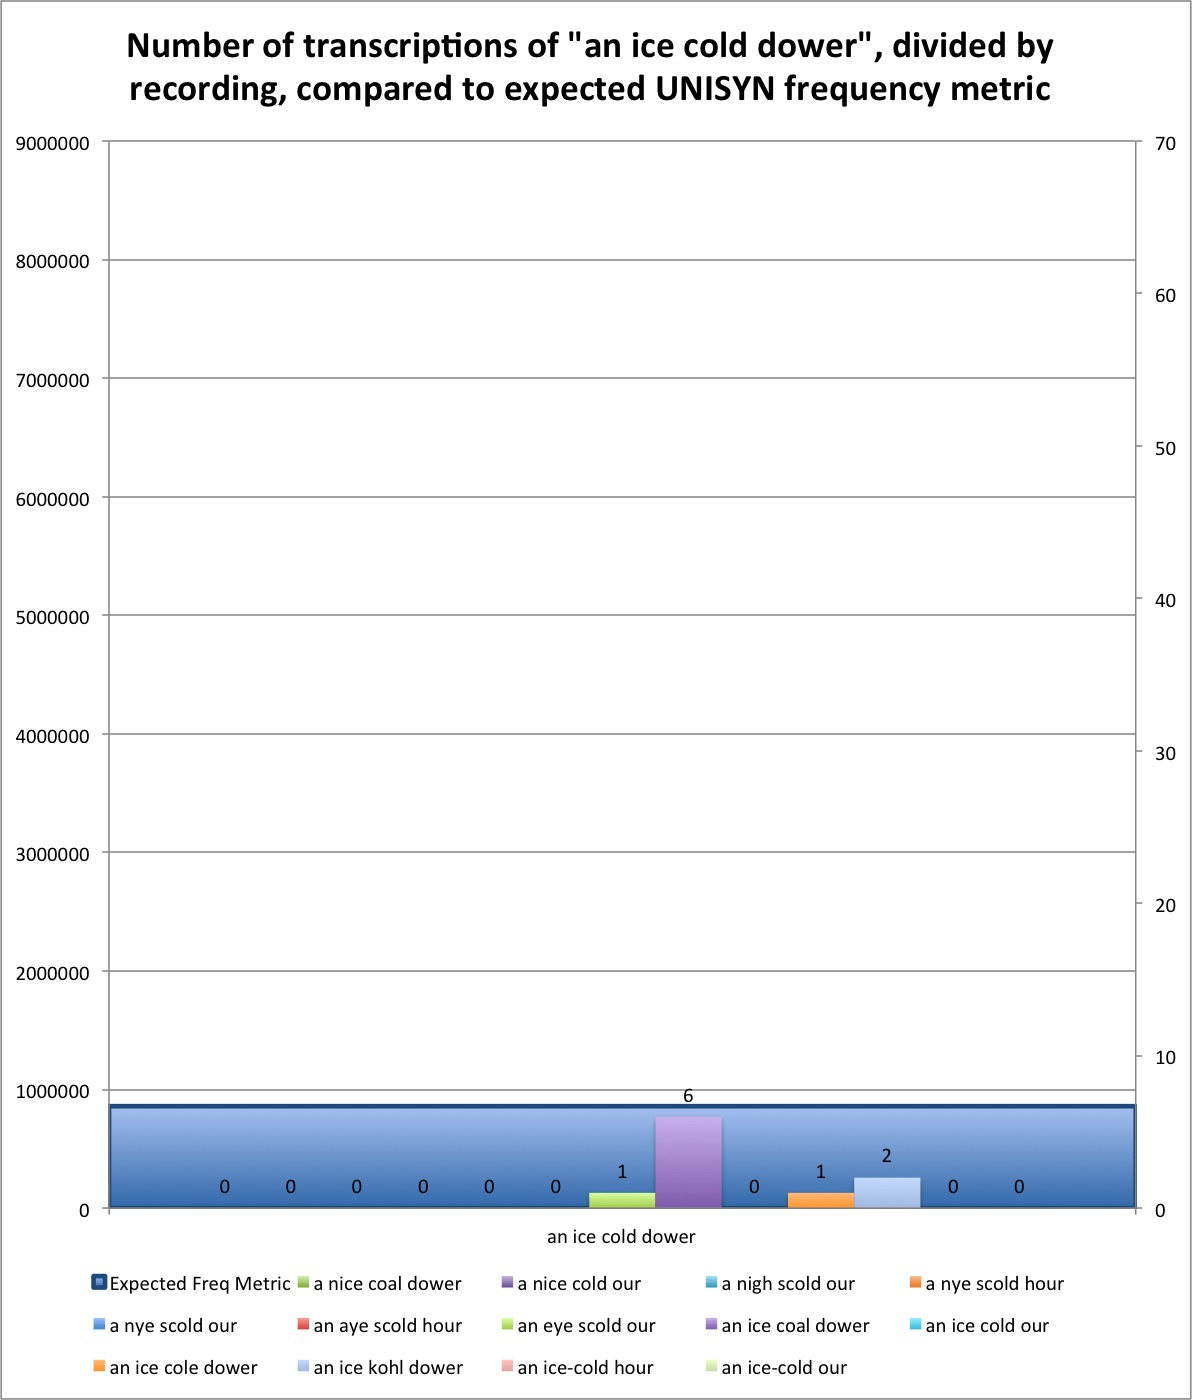
\includegraphics[width=\textwidth]{TranscriptionCountPerRecording_anIceColdDower.jpg}
\captionfonts
\caption[Transcription Count Per Recording for the transcribed phrase ``a nice cold dower'']{ This graph represents all transcriptions of the phrase ``a nice cold dower'', divided into columns based on what recording were transcribed as ``a nice cold dower''. The large blue bar in the background shows the predicted frequency metric for the phrase in question.}
\label{fig:results:transcriptionCountPerRecordingANiceColdDower}
\end{figure}


\subsubsection{An eye scold hour}
\label{results:transcriptionCountPerRecording:an_eye_scold_hour}

The chart for ``an eye scold hour'', shown in figure ~\ref{fig:results:transcriptionCountPerRecordingAnEyeScoldHour}, is primarily interesting in that it appears more or less deterministically interpretable. The only recordings that resulted in this phrase were those for ``an eye scold hour'' or ``an aye scold hour''. We hypothesize that this has something to do with word emphases, and suggest investigating this for future work. Interestingly enough, the predicted frequency value (scaled) was fairly close to the actual occurance for that phrase.


\begin{figure}
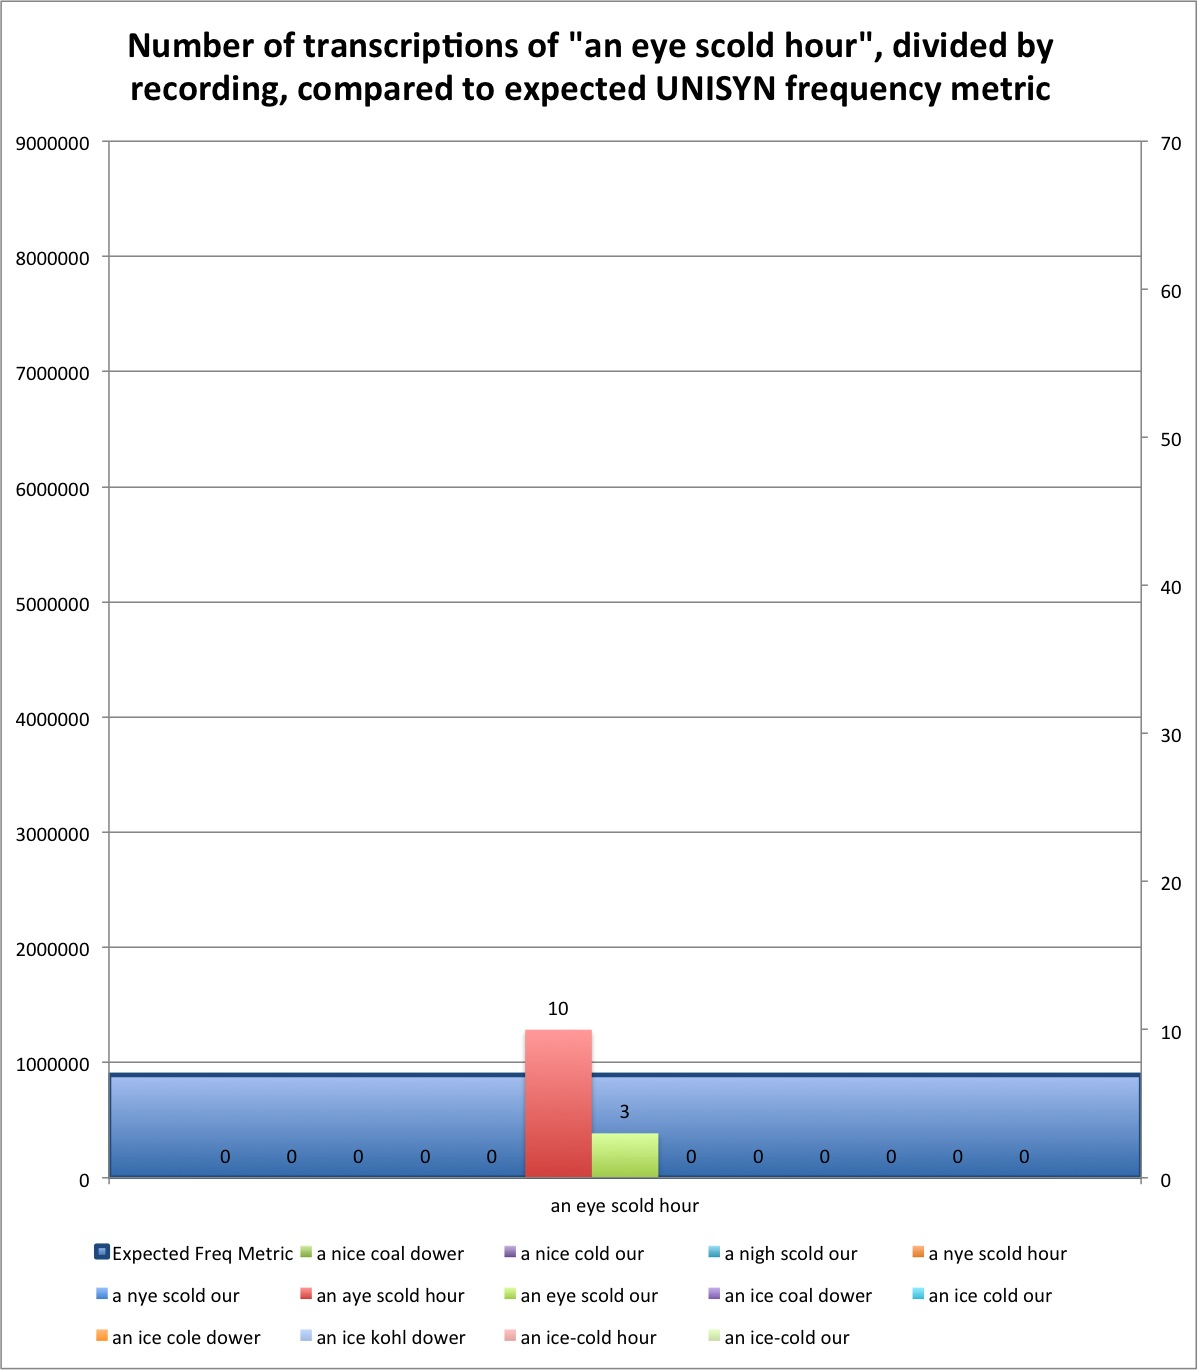
\includegraphics[width=\textwidth]{TranscriptionCountPerRecording_anEyeScoldHour.jpg}
\captionfonts
\caption[Transcription Count Per Recording for the transcribed phrase ``an eye scold hour'']{ This graph represents all transcriptions of the phrase ``an eye scold hour'', divided into columns based on what recording were transcribed as ``an eye scold hour''. The large blue bar in the background shows the predicted frequency metric for the phrase in question.}
\label{fig:results:transcriptionCountPerRecordingAnEyeScoldHour}
\end{figure}

\subsubsection{An ice coal dower}
\label{results:transcriptionCountPerRecording:an_ice_coal_dower}

The chart for ``an ice coal dower'' in figure ~\ref{fig:results:transcriptionCountPerRecordingAnIceCoalDower} is notable in that all its transcriptions came from recordings that began in ``an'' and ended in ``dower'', like the phrase itself does. As in ~\ref{fig:results:transcriptionCountPerRecordingAnEyeScoldHour}, we suggest that the near-deterministic interpretation has something to do with emphases, and suggest investigating this for future work. The UNISYN frequency metric once again predicted higher expected incidences than were actually observed for this transcription.

\begin{figure}
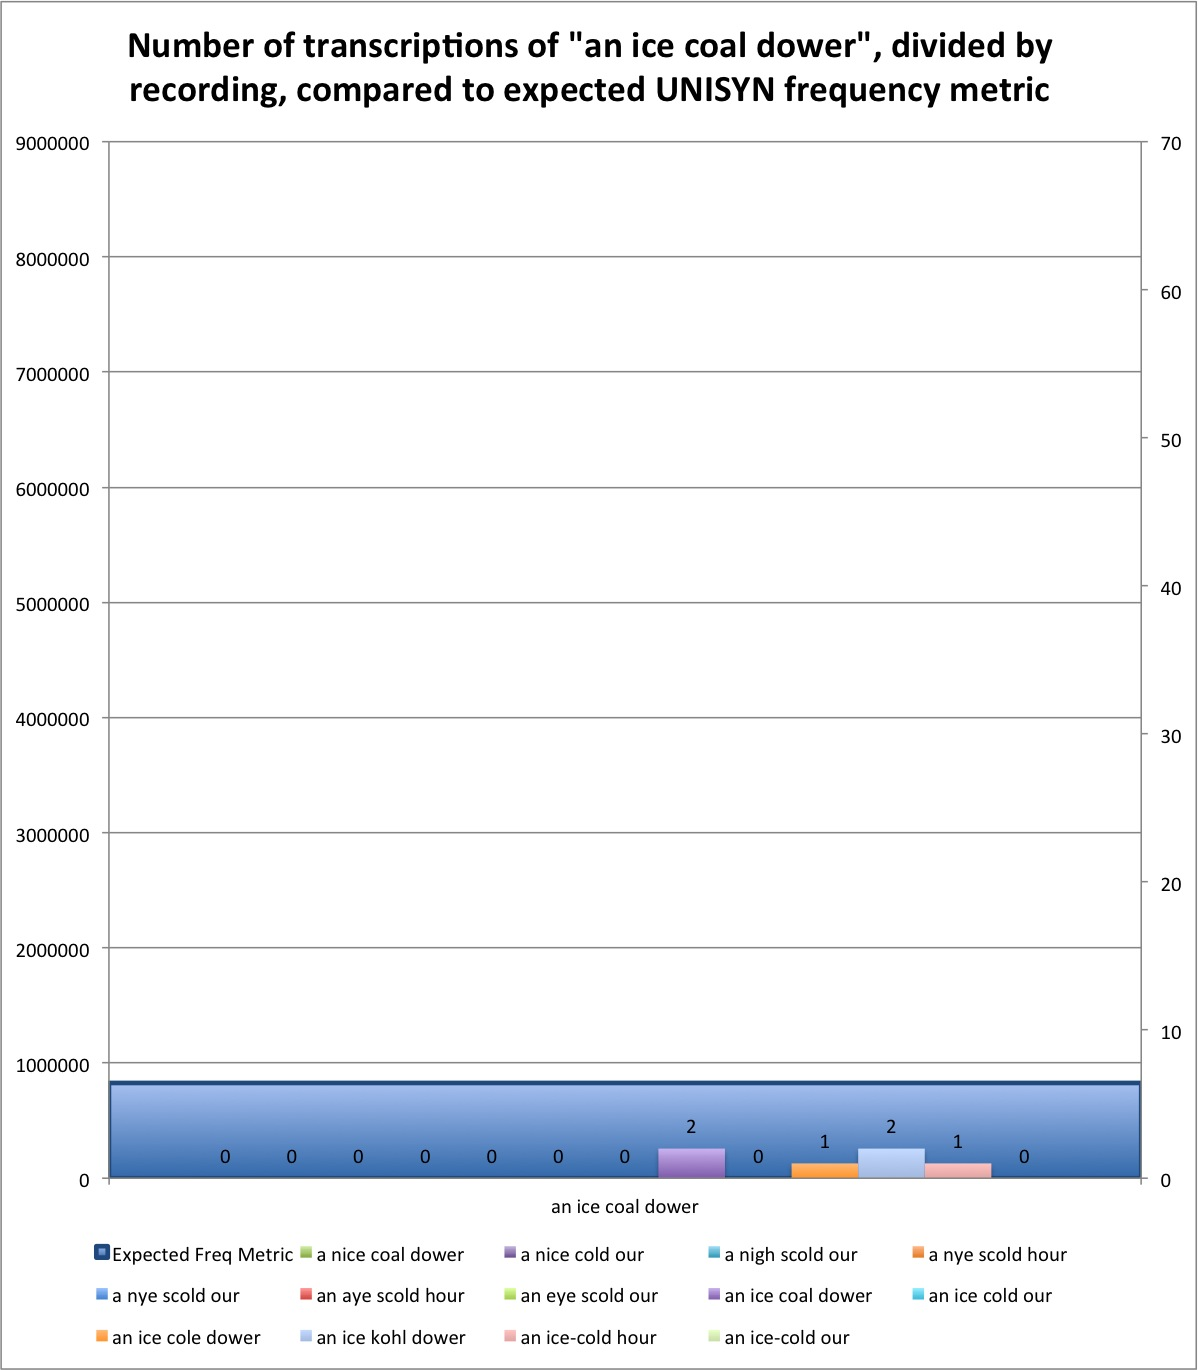
\includegraphics[width=\textwidth]{TranscriptionCountPerRecording_anIceCoalDower.jpg}
\captionfonts
\caption[Transcription Count Per Recording for the transcribed phrase ``an ice coal dower'']{ This graph represents all transcriptions of the phrase ``an ice coal dower'', divided into columns based on what recording were transcribed as ``an ice coal dower''. The large blue bar in the background shows the predicted frequency metric for the phrase in question.}
\label{fig:results:transcriptionCountPerRecordingAnIceCoalDower}
\end{figure}







\subsection{Transcription Breakdown By Country}
\label{results:transcriptionsByCountry}


When comparing transcriptions from countries where English is the dominant language (as shown in figure ~\ref{fig:results:EnglishDominantPieChart}) to those from countries where it is not (as shown in figure ~\ref{fig:results:NonNativePieChart}), we can make some interesting observations.  

\begin{figure}
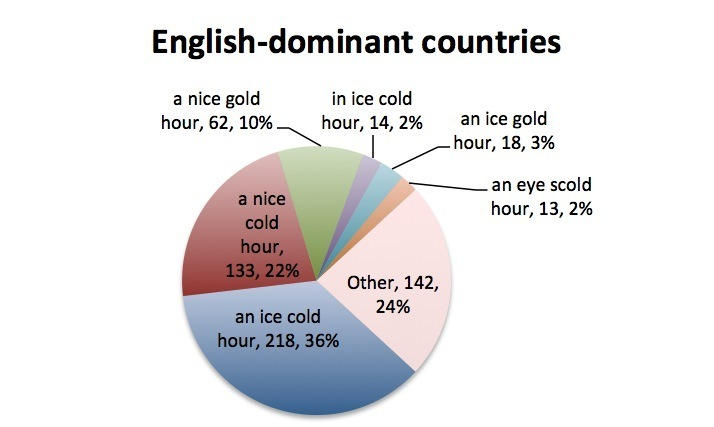
\includegraphics[width=\textwidth]{PieChart-EnglishDominantCountries-nobar.jpg}
\captionfonts
\caption[Pie Chart of transcriptions from countries that are primarily English-speaking]{ Pie Chart of transcriptions from countries that are primarily English-speaking.}
\label{fig:results:EnglishDominantPieChart}
\end{figure}

\begin{figure}
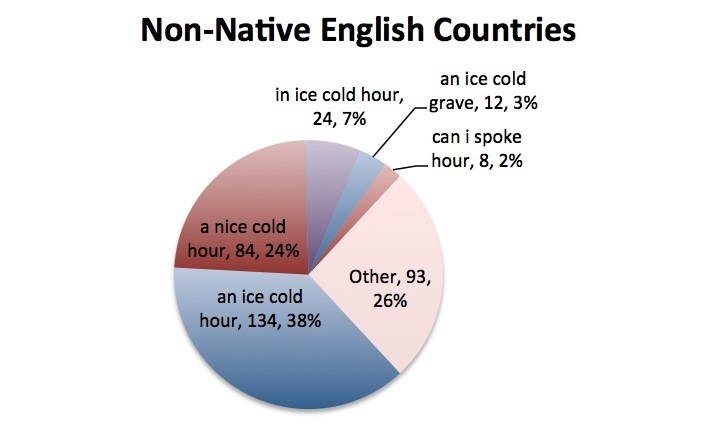
\includegraphics[width=\textwidth]{PieChart-NonNativeEnglishCountries-nobar.jpg}
\captionfonts
\caption[Pie Chart of transcriptions from countries that are Non-native English speakers]{ Pie Chart of transcriptions from countries that are Non-native English speakers.}
\label{fig:results:NonNativePieChart}
\end{figure}

\begin{enumerate}

\item The most common transcription for both is ``an ice cold hour'', with \percentTranscriptionsPerCountryAnIceColdHourEnglishDominant\% native-speaker transcriptions ( \transcriptionsPerCountryAnIceColdHourEnglishDominant) and \percentTranscriptionsPerCountryANiceColdHourNonNative\% non-native ( \transcriptionsPerCountryAnIceColdHourNonNative).

\item The second most common transcription is also the same for both (``a nice cold hour''), but it accounts for a larger percentage of the non-native pie ( \percentTranscriptionsPerCountryANiceColdHourNonNative\% compared to the native \percentTranscriptionsPerCountryANiceColdHourEnglishDominant\% ).

\item The third most common transcription differs for native and non-native speakers. 

Native speakers transcribed ``a nice gold hour'' \transcriptionsPerCountryANiceGoldHourEnglishDominant times, accounting for \percentTranscriptionsPerCountryANiceGoldHourEnglishDominant\% of all native transcriptions. In comparison, only \transcriptionsPerCountryANiceGoldHourNonNative non-native speaker transcribed that phrase, for a measley \percentTranscriptionsPerCountryANiceGoldHourNonNative\% of total non-native transcriptions. 

This brings up an interesting data point---the third most popular transcription for native speakers barely shows up at all for non-native transcribers. There may be something about common phoneme substitution that native speakers pick up on that non-natives do not; specifically, a cold/gold merger.  

 The third most common transcription for non-native speakers is ``in ice cold hour'', which was transcribed \transcriptionsPerCountryInIceColdHourNonNative times, and makes up \percentTranscriptionsPerCountryInIceColdHourNonNative\% of non-native transcriptions.  This phrase was the fifth most common transcription for native speakers, with \transcriptionsPerCountryInIceColdHourEnglishDominant transcriptions making up \percentTranscriptionsPerCountryInIceColdHourEnglishDominant\% of total transcriptions.  

\item The fourth most common transcription for native speakers was ``an ice gold hour'', getting \percentTranscriptionsPerCountryAnIceGoldHourEnglishDominant\% of the total with \transcriptionsPerCountryAnIceGoldHourEnglishDominant transcriptions (by 14 unique transcribers).  This phrase was not transcribed by any non-native speakers. This exhibits the same phone/phoneme substitution that we saw with ``a nice gold hour''.

The fourth most common phrase for non-native speakers, ``an ice cold grave'', was only transcribed by one unique worker, and as such, is not going to be taken into serious consideration. The fifth most common phrase, ``can I spoke hour'', was also only transcribed by one unique worker, and so also cannot be taken into serious consideration.


\end{enumerate}



\begin{table}
\begin{center}

\begin{tabular}{|c|c|c|c|c|c|c|}
\hline 
&
\multicolumn{2}{c|}{Some Data}&
&
\multicolumn{2}{c|}{Some More Data}&
\tabularnewline
\hline
\hline 
&  Hi-Res&  Lo-Res&  Reduction&  Hi-Res&  Lo-Res&  Speedup
\tabularnewline
\hline 
Row Data A &  225,467&  43,850&  80.6\%&  360&  90&  4.0
\tabularnewline
\hline 
Row Data B &  225,467&  16,388&  92.7\%&  360&  26&  13.8
\tabularnewline
\hline 
\end{tabular}


\captionfonts
\caption[Performance data]{Here is some performance data for the system.}
\label{table:performance}
\end{center}
\end{table}


LaTeX is a document markup language and document preparation system for the TeX typesetting program.

It is widely used by mathematicians, scientists, philosophers, engineers, and scholars in academia and the commercial world, and by others as a primary or intermediate format (e.g. translating DocBook and other XML-based formats to PDF) because of the quality of typesetting achievable by TeX. It offers programmable desktop publishing features and extensive facilities for automating most aspects of typesetting and desktop publishing, including numbering and cross-referencing, tables and figures, page layout and bibliographies.

LaTeX is intended to provide a high-level language to access the power of TeX. LaTeX essentially comprises a collection of TeX macros, and a program to process LaTeX documents. Since TeX's formatting commands are very low-level, it is usually much simpler for end-users to use LaTeX.

LaTeX was originally written in 1984 by Leslie Lamport at SRI International and has become the dominant method for using TeX�few people write in plain TeX anymore.

LaTeX is based on the idea that authors should be able to focus on the meaning of what they are writing, without being distracted by the visual presentation of the information. In preparing a LaTeX document, the author specifies the logical structure using familiar concepts such as chapter, section, table, figure, etc., and lets the LaTeX system worry about the presentation of these structures. It therefore encourages the separation of layout from content, while still allowing manual typesetting adjustments where needed. This is similar to the mechanism by which many word processors allow styles to be defined globally for an entire document, or the CSS mechanism used by HTML.

LaTeX can be arbitrarily extended by using the underlying macro language to develop custom formats. Such macros are often collected into packages which are available to address special formatting issues such as complicated mathematical content or graphics. In addition, there are numerous commercial implementations of the entire TeX system, including LaTeX, to which vendors may add extra features like additional typefaces and telephone support. LyX is a free visual document processor that uses LaTeX for a back-end. TeXmacs is a free, WYSIWYG editor with similar functionalities as LaTeX, but a different typesetting engine.

A number of popular commercial desktop publishing systems use modified versions of the original TeX typesetting engine. The recent rise in popularity of XML systems and the demand for large-scale batch production of publication-quality typesetting from such sources has seen a steady increase in the use of LaTeX.


% ------------- End main chapters ----------------------

\clearpage
\bibliography{examplebibliography}
\bibliographystyle{plain}
%\addcontentsline{toc}{chapter}{Bibliography}

\end{document}